\documentclass[12pt]{article}


\usepackage[dvips,letterpaper,margin=0.75in,bottom=0.5in]{geometry}
\usepackage{cite}
\usepackage{slashed}
\usepackage{graphicx}
\usepackage{amsmath}

\begin{document}

\title{Introduction to DC Circuits and Laboratory Equipment}

\maketitle

\section{Pre-lab Calculations}

For each of the calculations below, first calculate a general formula, then evaluate your formula for the specific component values listed in this lab description.  Specify the direction (e.g. up or down in the diagram) of currents.

1) For Fig.~\ref{fig:dividers}, calculate the voltage at point $V_{\rm out}$ in (a) and the current through resistors $R_1$ and $R_2$ in (b).

2) Calculate the voltage at points $P_1$, $P_2$, and $P_3$ and the current through resistors $R_1$, $R_2$ and $R_3$ for the circuit in Fig.~\ref{fig:loops}

3) Calculate the Th\'{e}venin equivalents for both circuits in Fig.~\ref{fig:thev}

\section{Introduction}

In this lab, you will become familiar with some essential electronics lab equipment:  voltage supplies, bread boards, digital multimeter (DMM), and function generator.  You will experimentally verify the DC circuit analysis techniques which we have developed in class.

\section{Resistors in Series and Parallel}

The one circuit you will most frequently encounter in life is the humble voltage divider, shown in Fig.~\ref{fig:dividers}a.  Build a divider with $V_1=10~V$, $R_1=8.2~\rm{k\Omega}$.  Measure $V_{\rm out}$ for values $R_2=3.9$, $8.2$ and $15~\rm{k\Omega}$.

Using the same components, build the current divider shown in Fig.~\ref{fig:dividers}b with $V_1=10~V$, $R_1=8.2~\rm{k\Omega}$.  Using your DMM as an ammeter (current measurement device) measure the current through $R_1$ and $R_2$ for with $R_2=3.9$, $8.2$ and $15~\rm{k\Omega}$.  Make sure to measure the magnitude and direction of the current (up or down in the diagram) and remember that to use your DMM as an ammeter, you must pass the current through the meter.

As we will learn, one sign of a poorly design circuit is a strict requirement on the value of a particular component, such as a resistor.  But what do you do when you don't have the exact value of a resistor that you need?  An old timer's trick (of somewhat dubious utility considering that 0.1\% tolerance resistors cost about six cents) is to trim down a standard E12 resistor by adding a larger resistor in parallel.  Trim your $8.2~\rm{k\Omega}$ resistor to achieve a resistance of $5.0\pm0.1~\rm{k\Omega}$.
%TODO:  add Fig.~\ref{fig:serpar} if more is needed.

\begin{figure}[htbp]
\begin{center}
\begin{tabular}{c@{\hskip 1in}c}
\begin{picture}(110,110)
\put(0,0){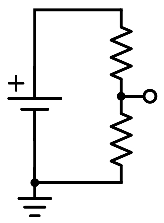
\includegraphics[height=0.15\textheight]{figs/rser.pdf}} 
\put(-8,45){$V_1$}
\put(35,35){$R_2$}
\put(35,79){$R_1$}
\put(80,55){$V_{\rm out}$}
\end{picture}
&
\begin{picture}(110,110)
\put(0,0){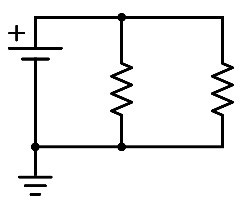
\includegraphics[height=0.15\textheight]{figs/rpar.pdf}}
\put(-5,65){$V_1$}
\put(42,55){$R_1$}
\put(93,55){$R_2$}
\end{picture}\\
(a) & (b) \\
\end{tabular}
\end{center}
\caption{\label{fig:dividers} Circuit diagrams for (a) a voltage divider circuit and (b) a current divider circuit.}
\end{figure}

%\begin{figure}[htbp]
%\begin{center}
%\begin{picture}(125,135)
%\put(0,0){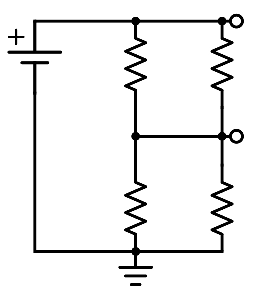
\includegraphics[height=0.20\textheight]{figs/rserpar.pdf}} 
%\put(-8,100){$V_1$}
%\put(40,35){$R_2$}
%\put(40,100){$R_1$}
%\put(85,35){$R_4$}
%\put(85,100){$R_3$}
%\put(120,120){$P_2$}
%\put(120,80){$P_1$}
%\end{picture}
%\end{center}
%\caption{\label{fig:serpar} Circuit diagram with resistors in series and parallel.}
%\end{figure}

\section{DC Circuit Analysis}

Build the circuit shown in Fig.~\ref{fig:loops} with components $V_1=10~\rm{V}$, $V_2=5~\rm{V}$, 
$R_1=3.3~\rm{k\Omega}$, $R_2=3.9~\rm{k\Omega}$, and $R_3=8.2~\rm{k\Omega}$.
Measure the voltages at points $P_1$,$P_2$ and $P_3$ and the currents (magnitude and direction) through each resistor.  Show that these match the results from circuit analysis, and explicitly verify Kirchhoff's voltage law through three loops and Kirchhoff's current law at two three-way junctions.
 
\begin{figure}[htbp]
\begin{center}
\begin{picture}(220,160)
\put(0,0){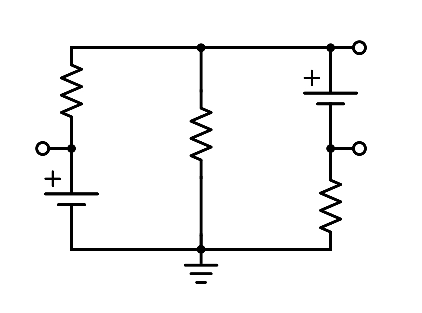
\includegraphics[height=0.25\textheight]{figs/dc_circuit.pdf}} 
\put(5,85){$P_1$}
\put(10,50){$V_1$}
\put(50,120){$R_1$}
\put(85,100){$R_2$}
\put(160,55){$R_3$}
\put(160,110){$V_2$}
\put(210,140){$P_3$}
\put(210,95){$P_2$}
\end{picture}
\end{center}
\caption{\label{fig:loops} Circuit diagram with resistors in series and parallel.}
\end{figure}

\section{Th\'{e}venin Equivalent Circuits}

Build the circuit shown in Fig.~\ref{fig:thev}a with $V_1=5~\rm{V}$, $V_2=15~\rm{V}$, 
$R_1=12~\rm{k\Omega}$ and $R_2=27~\rm{k\Omega}$.

Measure the short-circuit current and the open circuit voltage between $P_1$ and $P_2$, and confirm that this matches your calculation for the Th\'{e}venin Equivalent circuit.  Choose three appropriate resistance values (a sketch of the IV curve for the Th\'{e}venin circuit will help) to confirm the linear response of the circuit.


Sometimes the short-circuit current is purely theoretical.  If you attempt to short circuit points $P_1$ and $P_2$ for the circuit in Fig.~\ref{fig:thev}b you will \textit{destroy your ammeter.}  \textbf{So don't do that!}
Build the circuit in Fig.~\ref{fig:thev}b $V_1=5~\rm{V}$ and $R_1=3.3~\rm{k\Omega}$.
\textbf{Then, do not measure the short-circuit current!}  Instead, measure the open circuit voltage, as well as the voltage for three resistances in the range from $1~\rm{k\Omega}$ to $10~\rm{M\Omega}$.

\begin{figure}[htbp]
\begin{center}
\begin{tabular}{c@{\hskip 1in}c}
\begin{picture}(140,120)
\put(0,0){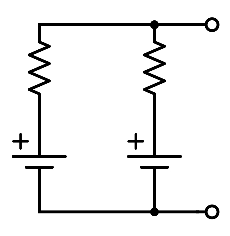
\includegraphics[height=0.18\textheight]{figs/theva.pdf}} 
\put(-8,35){$V_1$}
\put(30,80){$R_1$}
\put(92,80){$R_2$}
\put(55,35){$V_2$}
\put(110,20){$P_1$}
\put(110,100){$P_2$}
\end{picture}
&
\begin{picture}(140,120)
\put(0,0){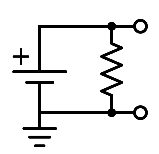
\includegraphics[height=0.12\textheight]{figs/thevb.pdf}}
\put(-3,27){$V_1$}
\put(38,45){$R_1$}
\put(83,60){$P_2$}
\put(83,20){$P_1$}
\end{picture}\\
(a) & (b) \\
\end{tabular}
\end{center}
\caption{\label{fig:thev} Diagrams for determining Th\'{e}venin equivalent circuits.  Be careful with circuit (b):  if you short circuit the points $P_1$ and $P_2$ you will \textit{destroy your ammeter}. \textbf{So don't do that!}}
\end{figure}

\section{Limitations of Test Equipment}

Ideally, your DMM would not effect the circuit you are measuring at all, but this is not the case.
An ideal ammeter has zero resistance (no voltage change as the current passes through unaffected) and an ideal voltmeter has infinite resistance (no effect from parallel resistance when measuring across two points).  In reality, your DMM has a small non-zero resistance when used as an ammeter, and a large (but non-infinite) resistance when used as a voltmeter.

Build the voltage divider of Fig.~\ref{fig:dividers}a but with $V_1=10~\rm{V}$ and $R_1 = R_2 = 10~\rm{M\Omega}$.  Compare the value your measure with what you predict.  Calculate the resistance of your voltmeter.

%\section{Measuring Alternating Current with the DMM}
%
%Set your function generator to $50~\rm{\Omega}$ termination (which is usually the default).  Then, setup your function generator to produce a $1~\rm{V}$ peak-to-peak square wave across a $50~\rm{\Omega}$ resistor.  Using your DMM, measure the AC RMS voltage across the resistor.  Now change the function generator to provide a sine wave, but leave the amplitude unchanged.  Measure the AC RMS voltage across the resistor.  By what factor do these two measurements differ?  Does that value make sense?
%
%Repeat these two measurements using an $82~\rm{k\Omega}$ resistor.  Then, set your function generator to high impedance termination, and repeat one last time.   Using your knowledge of voltage dividers, can you figure out what is going on?

\section{Lab Report}

You should include all measurements made in this lab and compare them to your calculated values.  For the Th\'{e}venin equivalent circuits, also provide IV curves showing your measured values as points.  Answer the questions posed in the text.
 
\end{document}
